% vim: set tw=78 sts=2 sw=2 ts=8 aw et:
\documentclass{so.cs.pub.ro}

\usepackage{code/highlight}

\title[Laborator 1]{Laborator 1}
\subtitle{Introducere}
\date{25 Februarie - 2 Martie 2016}

\begin{document}

\frame{\titlepage}

\begin{frame}{Cine sunt?}
  \begin{itemize}    % Just like normal LaTeX
    \item email
    \item experienţă
    \item pasiuni relevante
    \item de ce SO?
    \end{itemize}		
\end{frame}

\begin{frame}{Resurse}
	\begin{itemize}
		\item Wiki: http://ocw.cs.pub.ro/so
		\begin{itemize}
			\item NeedToKnow page: http://ocw.cs.pub.ro/so/meta/need-to-know
			\item Folosiți feed-ul RSS 
		\end{itemize}
		\item Lista de discuții
		\begin{itemize} 
			\item so@cursuri.cs.pub.ro
			\item Abonați-vă (detalii pe wiki)
		\end{itemize}
		\item Catalog Google, calendar Google
		\item Mașini virtuale
		\item vmchecker (verificare teme)
		\item Documentație
		\item cs.curs.pub.ro (rol de portal + workshop)
		\item Pagină de Facebook
	\end{itemize}
\end{frame}

\begin{frame}{Despre laborator}
  	\begin{itemize}   
    		\item Subiecte principale
		\begin{itemize}
			\item Procese
			\item Thread-uri
			\item Comunicare și sincronizare
			\item Memorie
			\item Sisteme de fișiere
			\item I/O
		\end{itemize}
		\vspace*{0.2cm}
		\item POSIX/Win32 API programming (C/C++)
		\item 7 minute workshop / 15 min prezentare / restul task-uri
		\item Tutorial-like, task-based, learn by doing
		\item Karma Points ("pentru cei puternici")
    	\end{itemize}		
\end{frame}

\begin{frame}{Workshop}
  	\begin{itemize}   
    		\item Testul
		\begin{itemize}
			\item 3 întrebări din laboratorul curent
			\item Primele 7 minute din laborator
			\item Întrebări atât teoretice, cât și practice
		\end{itemize}
		\item Punctare
		\begin{itemize}
			\item Corectați voi: acasă, random și anonim câte două teste; deadline: o săptămână după încheierea laboratorului
			\item Nota finală pe test: punctajul primit pe test (50\%) + punctaj pe cum ați corectat (50\%)
		\end{itemize}
		\item Total teste: 5 (la începutul laboratoarelor 2, 4, 6, 8, 11)
    	\end{itemize}		
\end{frame}

\begin{frame}{Teme}
  	\begin{itemize}   
    		\item Tema 0 – hash-table
		\item Tema 1 – mini-shell
		\item Tema 2 – demand pager/swapper
		\item Tema 3 – thread scheduler
		\item Tema 4 – server de fișiere
		\vspace*{0.2cm}
		\item Intense
		\item Necesare: aprofundare API (laborator) și concepte (curs)
		\item Estimare de timp: 8-20 ore pe temă
		\item Teste publice
		\item Suport de testare la submit - feedback imediat
    	\end{itemize}		
\end{frame}

\begin{frame}{Reguli și notare}
  	\begin{itemize}
        \item http://ocw.cs.pub.ro/courses/so/meta/notare/reguli-notare-cb  
		\item Examen final - 4 puncte
    		\item Activitate laborator - 1 punct
		\begin{itemize}
			\item 0.75 puncte workshop, 0.75 puncte task-uri =$>$ trunchiere la 1 punct
			\item Prezență activă obligatorie la cel puțin 8 laboratoare pentru a intra în examen
		\end{itemize}
	\end{itemize}
\end{frame}

\begin{frame}{Reguli și notare (2)}
  	\begin{itemize}  
		\item Teme - 5 puncte + 4 puncte * corelare punctaj
		\begin{itemize}
			\item Fiecare temă valorează 1punct
			\item Rezolvată pe ambele platforme, fiecare temă este punctată cu maxim 1 punct, punctajele se cumulează și se trunchiază la 1 punct.
			\item Trunchiere la 5 puncte pentru teme 
		\end{itemize}
		\item Depunctare teme
		\begin{itemize}
			\item -0.25 puncte pe zi (din 10) timp de 14 zile
			\item După 14 zile tema nu se mai punctează
		\end{itemize}
		\item Punctajul de absolvire a cursului este 4.5
		\item După restanțe tot punctajul se resetează la 0
    	\end{itemize}		
\end{frame}

\begin{frame}{Karma Awards}
  	\begin{itemize}   
    		\item Cum se obțin Karma Points?
		\begin{itemize}
			\item Participare la discuțiile din timpul cursului
			\item Participare la discuțiile din timpul laboratorului
			\item Răspunsuri pe lista de discuții
			\item Editarea wiki-ului
			\item Exercițiile bonus din timpul laboratorului
			\item Teme elegante
			\begin{itemize}
				\item Coding style consistent, comentarii punctuale, claritatea codului
				\item Soluții simple și corecte
				\item Modularitate, cursivitate 
			\end{itemize}
		\end{itemize}
    	\end{itemize}		
\end{frame}


\begin{frame}{Desfășurare laborator}
	\begin{itemize}
		\item Parcurgere laborator acasă -  40 de minute
		\item Workshop - 7 minute
		\item Prezentare teoretică + întrebări - 15 de minute
		\item Rezolvare exerciții - 80 de minute
		\begin{itemize}
	    		\item Punctaj între 0 și 11
	   		 \item Bucuria rezolvării unui laborator de SO infinită :)
		\end{itemize}
		\item Workshop
		\begin{itemize}
	    		\item 3 întrebări din laboratorul curent
		\end{itemize}
	\end{itemize}
\end{frame}

\begin{frame}{Suport de laborator}
	\begin{itemize}
	\item Cărți
	\begin{itemize}
		\item TLPI, The Linux Programming Interface, M. Kerrisk
		\item WSP4, Windows System Programming 4th Edition, J. Hart
	\end{itemize}
	\item Listă de discuții
	\begin{itemize}
		\item http://cursuri.cs.pub.ro/cgi-bin/mailman/listinfo/so
	\end{itemize}
	\item Canal IRC, rețea Freenode, \#cs\_so
	\end{itemize}
\end{frame}

\begin{frame}{Ce vom învăța în laborator}
	\begin{itemize}
		\item Compilare, depanare, biblioteci
		\item Operații I/E simple
		\item Procese
		\item Gestiunea memoriei
		\item Comunicarea inter-procese
		\item Semnale 
		\item Memoria virtuală
		\item Fire de execuție (2) 
		\item Operații de I/E avansate (2)
		\item Profiling 
		\item Securitate
	\end{itemize}
\end{frame}

\begin{frame}{Laboratorul 1}
	\begin{itemize}
		\item Compilare
		\begin{itemize}
			\item Traducerea unui program (limbaj sursă, limbaj țintă)
		\end{itemize}
		\item {Makefile}
		\begin{itemize}
			\item Automatizarea procesului de compilare
		\end{itemize}
		\item Depanare
		\begin{itemize}
			\item Detectarea erorilor din programe
		\end{itemize}
		\item Biblioteci
		\begin{itemize}
			\item Colecție de fișiere precompilate
		\end{itemize}
	\end{itemize}
\end{frame}

\begin{frame}{Fazele compilării}
	\begin{figure}[htb]
		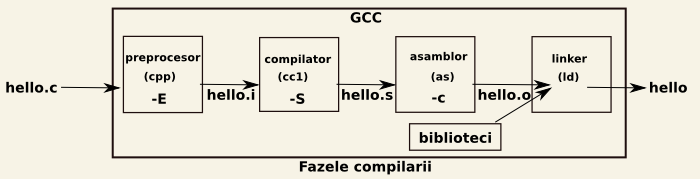
\includegraphics[width=11cm]{code/compilation-phases.png}
	\end{figure}
\end{frame}

\begin{frame}{GCC}
	\begin{itemize}
		\item GNU Compiler Collection
		\item gcc hello.c
		\begin{itemize}
			\item Compilare simplă, rezultă fișierul executabil a.out
		\end{itemize}
		\item gcc hello.c -o hello
		\begin{itemize}
			\item Compilare simplă cu specificarea numelui fișierului de ieșire
		\end{itemize}
		\item gcc hello.c -c -o hello.o
		\begin{itemize}
			\item Oprirea compilării după obținerea fișierului obiect
		\end{itemize}
		\item gcc hello.o -o hello
		\begin{itemize}
			\item Editarea de legături pentru fișierul obiect hello.o
		\end{itemize}
	\end{itemize}
\end{frame}

\begin{frame}{cl}
	\begin{itemize}
		\item cl.exe - Microsoft Compiler
		\item cl hello.c
		\begin{itemize}
			\item Compilare simplă, rezultă fișierul executabil hello.exe
		\end{itemize}
		\item cl /Fehello\_win.exe hello.c
		\begin{itemize}
			\item Compilare simplă cu specificarea numelui executabilului
		\end{itemize}
		\item cl /c hello.c
		\begin{itemize}
			\item Obținerea fișierului obiect
		\end{itemize}
		\item cl /Fehello.obj
		\begin{itemize}
			\item Editarea de legături pentru fișierul obiect
		\end{itemize}
		\item cl /? - help
	\end{itemize}
\end{frame}

\begin{frame}{Fișiere make}
	\begin{itemize}
		\item Automatizarea compilării
		\item Fișier Makefile
		\begin{itemize}
			\item Reguli
			\item Comenzi
			\item Variabile
		\end{itemize}
		\item Compilare 'deșteaptă'
		\item make vs. nmake
	\end{itemize}
\end{frame}

\begin{frame}{gdb}
	\begin{itemize}
		\item Fișierele sunt compilate cu opțiunea -g
		\item Execuție
		\begin{itemize}
			\item gdb ./a.out
		\end{itemize}
		\item Comenzi utile
		\begin{itemize}
			\item p - print
			\item bt - backtrace
			\item step, next
			\item set args
		\end{itemize}
	\end{itemize}
\end{frame}

\begin{frame}{Biblioteci}
	\begin{itemize}
		\item Statice
		\begin{itemize}
			\item Rezolvare simboluri în momentul editării de legături
			\item Funcțiile utilizate sunt incluse în executabil
			\item Dimensiune executabil mai mare, rulare mai rapidă
		\end{itemize}
		\item Dinamice
		\begin{itemize}
			\item Rezolvare simbolurilor se poate face
			\begin{itemize}
					\item La încărcare (load-time)
					\item La rulare (run-time) (dlopen and friends)
			\end{itemize}
			\item Executabil de dimensiune redusă
		\end{itemize}
	\end{itemize}
\end{frame}

\begin{frame}{Lucrul cu biblioteci în Linux}
	\begin{itemize}
		\item Crearea unei biblioteci statice (.a)
		\begin{itemize}
			\item ar rc libxyz.a f1.o f2.o
		\end{itemize}
		\item Crearea unei biblioteci partajate (.so)
		\begin{itemize}
			\item gcc -fPIC -c f1.c
			\item gcc -shared f1.o -o libxyz.so 
		\end{itemize}
		\item Legarea cu o bibliotecă
		\begin{itemize}
			\item -lxyz
			\item -L{path} 
			\item LD_LIBRARY_PATH
		\end{itemize}
	\end{itemize}
\end{frame}

\begin{frame}{Lucrul cu biblioteci în Windows}
	\begin{itemize}
			\item Crearea unei biblioteci statice (.lib)
			\begin{itemize}
				\item lib /out:$<$nume.lib$>$ $<$lista fisiere obiect$>$
			\end{itemize}
			\item Crearea unei biblioteci dinamice (.dll)
			\begin{itemize}
				\item __declspec(dllimport), __declspec(dllexport)
				\item link (/dll) sau cl /LD
			\end{itemize}
	\end{itemize}
\end{frame}

%\begin{frame}{Întrebări}
%\begin{itemize}
%\item Care este cea mai simplă comandă care compilează programul hello.c?
%\item De ce includerea de mai multe ori a unui fișier antet standard nu generează o eroare la compilare?
%\item Este posibil ca dimensiunea unui fișier după faza de preprocesare să fie mai mică decât a fișierului .c original?
%\end{itemize}
%\end{frame}




\end{document}
